\documentclass[aspectratio=169,11pt]{beamer}

% Presentación de Seminario de Título basada en main.tex
\usepackage[utf8]{inputenc}
\usepackage[T1]{fontenc}
% Babel en español cuando está instalado; fallback para TeX Live sin spanish.ldf.
\IfFileExists{spanish.ldf}{%
  \usepackage[spanish,es-noshorthands]{babel}%
  \spanishdecimal{.}%
}{%
  \usepackage[english]{babel}%
}
\usepackage{lmodern}
\usepackage{microtype}
\usepackage{amsmath,amssymb}
\usepackage{booktabs,tabularx,array,colortbl}
\usepackage{graphicx}
\usepackage{xcolor}
\usepackage{tikz}
\usetikzlibrary{shapes,arrows,arrows.meta,positioning,calc,fit,patterns,backgrounds}
\usepackage{pgfplots}
\pgfplotsset{compat=1.15}
\usepackage{csquotes}
\usepackage[
  backend=biber,
  style=authoryear-comp,
  maxcitenames=2,
  maxbibnames=8,
  giveninits=true,
  uniquename=init,
  doi=false,
  url=false,
  isbn=false
]{biblatex}
\addbibresource{referencias.bib}

% Estilo visual tomado de ejemplojessica.tex
\definecolor{primary}{RGB}{15,76,110}
\definecolor{accent}{RGB}{224,122,40}
\definecolor{best}{RGB}{0,128,64}
\definecolor{warn}{RGB}{183,65,14}
\definecolor{inkgray}{RGB}{55,55,60}
\definecolor{lightbg}{RGB}{236,242,246}

% Alias para mantener editables los diagramas y tablas existentes
\colorlet{PUCVBlue}{primary}
\colorlet{PUCVBlueDark}{primary}
\colorlet{PUCVLight}{lightbg}
\colorlet{PUCVRed}{warn}
\colorlet{GreenH}{best}
\colorlet{WarmGold}{accent}
\colorlet{Ink}{inkgray}
\colorlet{Muted}{inkgray!78}
\colorlet{PaleGray}{lightbg}

\usetheme{default}
\useinnertheme{circles}
\setbeamercolor{normal text}{fg=inkgray}
\setbeamercolor{structure}{fg=primary}
\setbeamercolor{title}{fg=primary}
\setbeamercolor{subtitle}{fg=inkgray}
\setbeamercolor{frametitle}{fg=white,bg=primary}
\setbeamercolor{block title}{fg=white,bg=primary}
\setbeamercolor{block body}{fg=inkgray,bg=lightbg}
\setbeamercolor{block title alerted}{fg=white,bg=warn}
\setbeamercolor{block body alerted}{fg=inkgray,bg=warn!8}
\setbeamercolor{block title example}{fg=white,bg=best}
\setbeamercolor{block body example}{fg=inkgray,bg=best!8}
\setbeamercolor{itemize item}{fg=accent}
\setbeamercolor{itemize subitem}{fg=accent}
\setbeamercolor{section in toc}{fg=primary}
\setbeamercolor{author in head/foot}{fg=white,bg=primary!85}
\setbeamercolor{bibliography entry author}{fg=inkgray}
\setbeamercolor{bibliography entry title}{fg=inkgray!78}
\setbeamercolor{bibliography entry location}{fg=inkgray!78}
\setbeamercolor{bibliography entry note}{fg=inkgray!78}

\setbeamerfont{title}{series=\bfseries,size=\LARGE}
\setbeamerfont{subtitle}{size=\normalsize}
\setbeamerfont{frametitle}{series=\bfseries,size=\large}
\setbeamerfont{footline}{size=\scriptsize}

\setbeamertemplate{blocks}[rounded][shadow=false]
\setbeamertemplate{navigation symbols}{}
\setbeamertemplate{itemize items}[circle]
\setbeamertemplate{bibliography item}{\raisebox{0.2ex}{\tiny$\blacksquare$}}

% Banda superior y pie, iguales al estilo del ejemplo
\setbeamertemplate{frametitle}{%
  \nointerlineskip
  \begin{beamercolorbox}[wd=\paperwidth,ht=3.0ex,dp=1.2ex,leftskip=0.35cm,rightskip=0.35cm]{frametitle}%
    \usebeamerfont{frametitle}\insertframetitle%
  \end{beamercolorbox}%
}

\setbeamertemplate{footline}{%
  \leavevmode%
  \hbox{%
    \begin{beamercolorbox}[wd=.72\paperwidth,ht=2.4ex,dp=1.1ex,leftskip=0.35cm]{author in head/foot}%
      \usebeamerfont{footline}Optimización cooperativa de HRES--H$_2$ \; · \; DTW/DDTW%
    \end{beamercolorbox}%
    \begin{beamercolorbox}[wd=.28\paperwidth,ht=2.4ex,dp=1.1ex,rightskip=0.35cm]{author in head/foot}%
      \usebeamerfont{footline}\hfill\insertframenumber\,/\,\inserttotalframenumber%
    \end{beamercolorbox}%
  }%
}

\newcommand{\smallcite}[1]{{\scriptsize\color{inkgray!72}\parencite{#1}}}
\newcommand{\key}[1]{\textcolor{primary}{\textbf{#1}}}
\newcommand{\risk}[1]{\textcolor{warn}{\textbf{#1}}}
\newcommand{\good}[1]{\textcolor{best}{\textbf{#1}}}
\newcommand{\destacado}[1]{\textcolor{primary}{\textbf{#1}}}
\newcommand{\gcell}{\cellcolor{primary!78}\color{white}\bfseries X}
\newcommand{\hcell}{\cellcolor{accent!24}\color{accent!70!black}\bfseries $\star$}

\title[Optimización cooperativa HRES-H2]{Desarrollo de arquitecturas híbridas para la optimización del HRES-H2 con tecnologías de hidrógeno verde}
\author{Lucas Erazo}
\institute{Escuela de Ingeniería Informática\\Pontificia Universidad Católica de Valparaíso\\[3pt]
\small Profesor guía: Emanuel Vega \qquad Profesor correferente: Ricardo Soto}
\date{Septiembre de 2026}

\begin{document}

% -----------------------------------------------------------------------------
\begin{frame}[plain]
  % Logos institucionales de la portada.
  \nointerlineskip
  \makebox[\textwidth][s]{\hspace{0.1cm}
    
\includegraphics[width=7.0cm]{fig/logo_100.png}\hfill
    
\includegraphics[height=1.7cm]{fig/Logo_pucv_ok.PNG}\hspace{0.1cm}}
  \vspace{0.25cm}
  \titlepage
\end{frame}

\begin{frame}{Estructura de la presentación}
  \tableofcontents
\end{frame}

\section{1. Problema y sistemas cooperativos}

\begin{frame}[plain]
  \centering
  \vfill
  {\usebeamerfont{title}\color{primary}1. Problema y sistemas cooperativos}\\[0.6em]
  {\color{accent}\rule{4.2cm}{2.2pt}}
  \vfill
\end{frame}

% -----------------------------------------------------------------------------
\begin{frame}{El desafío de coordinar la búsqueda}
  \begin{columns}[T,onlytextwidth]
    \column{0.48\textwidth}
      {\large\key{Exploración global}}
      \vspace{0.18cm}

      Recorre regiones distintas del espacio de soluciones y conserva diversidad.

      \vspace{0.45cm}
      {\large\key{Explotación local}}
      \vspace{0.18cm}

      Refina soluciones prometedoras y acelera la convergencia cerca de buenos óptimos.

    \column{0.48\textwidth}
      \begin{block}{Tensión principal}
        Demasiada exploración retrasa la convergencia. Demasiada explotación provoca convergencia prematura.
      \end{block}
      \vspace{0.3cm}

      El mejor comportamiento depende del problema y también de la etapa de cada ejecución.

      \vspace{0.25cm}
      \smallcite{wolpert1997no,vega2021learning,akbulut2026artificial}
  \end{columns}
\end{frame}

% -----------------------------------------------------------------------------
\begin{frame}{La decisión que controla el sistema híbrido}
  \vspace{0.1cm}
  \begin{block}{Pregunta central}
    ¿Cuándo debe terminar la fase del solucionador activo y transferir el control a otro algoritmo?
  \end{block}

  \vspace{0.35cm}
  \begin{tabularx}{\textwidth}{>{\bfseries\color{PUCVBlueDark}}p{3.25cm} X}
    Presupuesto fijo & Es simple, pero ignora la dinámica observada durante la ejecución. \\[0.25cm]
    Umbral manual & Depende de la escala del objetivo, el paisaje y el algoritmo monitoreado. \\[0.25cm]
    Indicador escalar & Resume el estado actual, pero puede confundir una meseta transitoria con estancamiento. \\[0.25cm]
    Política aprendida & Modela relaciones complejas, aunque requiere estados, entrenamiento y recompensas. \\
  \end{tabularx}

  \vfill
  \smallcite{talbi2021machine_tax,pei2025adaptive,adriaensen2022automated}
\end{frame}

% -----------------------------------------------------------------------------
\begin{frame}{Estado del arte: sistemas cooperativos}
  \vspace{0.18cm}
  \begin{tabularx}{\dimexpr\textwidth+0.15cm\relax}{>{\raggedright\arraybackslash}p{4.45cm} >{\raggedright\arraybackslash}X}
    \rowcolor{primary!14}
    \textcolor{PUCVBlueDark}{\textbf{Trabajo}} &
    \textcolor{PUCVBlueDark}{\textbf{Qué estudia o aporta}} \\
    \addlinespace[0.06cm]
    \textcolor{PUCVBlueDark}{\textbf{Żychowski et al. (2025)}} &
    \scriptsize Propone un portafolio de islas: metaheurísticas en paralelo intercambian soluciones y adaptan la migración. \\
    \addlinespace[0.07cm]
    {\textcolor{PUCVBlueDark}{\textbf{Drake et al. (2020)}}\newline
     \textcolor{PUCVBlueDark}{\textbf{Dokeroglu et al. (2024)}}} &
    \scriptsize Revisan hiperheurísticas: una capa superior selecciona, genera o secuencia métodos de búsqueda. \\
    \addlinespace[0.07cm]
    \textcolor{PUCVBlueDark}{\textbf{Derbel y Verel (2011)}} &
    \scriptsize DAMS permite que nodos distribuidos decidan qué metaheurística aplicar y qué información comunicar. \\
    \addlinespace[0.07cm]
    {\textcolor{PUCVBlueDark}{\textbf{Mambrini y Sudholt (2015)}}\newline
     \textcolor{PUCVBlueDark}{\textbf{Pei et al. (2025)}}} &
    \scriptsize Estudian cómo ajustar intervalos de migración o seleccionar operadores según las mejoras y el estado de búsqueda. \\
    \bottomrule
  \end{tabularx}

  \vspace{0.15cm}
  \centering
  {\scriptsize\destacado{Decisión de coordinación:} cuándo comunicar, qué transferir y qué solucionador continúa.}
\end{frame}

% -----------------------------------------------------------------------------
\begin{frame}{Brecha de investigación}
  \begin{columns}[T,onlytextwidth]
    \column{0.54\textwidth}
      La literatura ya utiliza:
      \begin{itemize}
        \item mejora reciente del fitness;
        \item diversidad y características de población;
        \item historiales de operadores;
        \item características de trayectorias para selección y \textit{warm-start}.
      \end{itemize}

      \vspace{0.25cm}
      \smallcite{jankovic2022trajectory,kostovska2022per,cenikj2026survey}

    \column{0.42\textwidth}
      \vspace{0.15cm}
      {\Large\color{PUCVRed}\bfseries Falta explotar de forma explícita la forma temporal del fitness incumbente}

      \vspace{0.5cm}
      La propuesta usa similitud de trayectorias para distinguir progreso sostenido de estancamiento persistente y gobernar el cambio de solucionador.
  \end{columns}
\end{frame}

\section{2. DTW/DDTW y arquitectura propuesta}

\begin{frame}[plain]
  \centering
  \vfill
  {\usebeamerfont{title}\color{primary}2. DTW/DDTW y detección de estancamiento}\\[0.6em]
  {\color{accent}\rule{4.2cm}{2.2pt}}
  \vfill
\end{frame}

% -----------------------------------------------------------------------------
\begin{frame}{Objetivo y alcance}
  \begin{block}{Objetivo general}
    Desarrollar y validar un marco cooperativo de metaheurísticas para dimensionar HRES--H$_2$, usando DTW/DDTW como detector adaptativo de estancamiento y como señal de coordinación.
  \end{block}

  \vspace{0.25cm}
  \begin{enumerate}
    \item Caracterizar el modelo, sus restricciones y no linealidades.
    \item Diseñar el detector sobre ventanas móviles del mejor fitness.
    \item Definir el intercambio de soluciones entre algoritmos heterogéneos.
    \item Orquestar la alternancia entre exploración y explotación.
    \item Validar el marco y extenderlo mediante $\varepsilon$-restricción adaptativa.
  \end{enumerate}
\end{frame}

% -----------------------------------------------------------------------------
\begin{frame}{Diagrama de flujo de la propuesta}
  \centering
  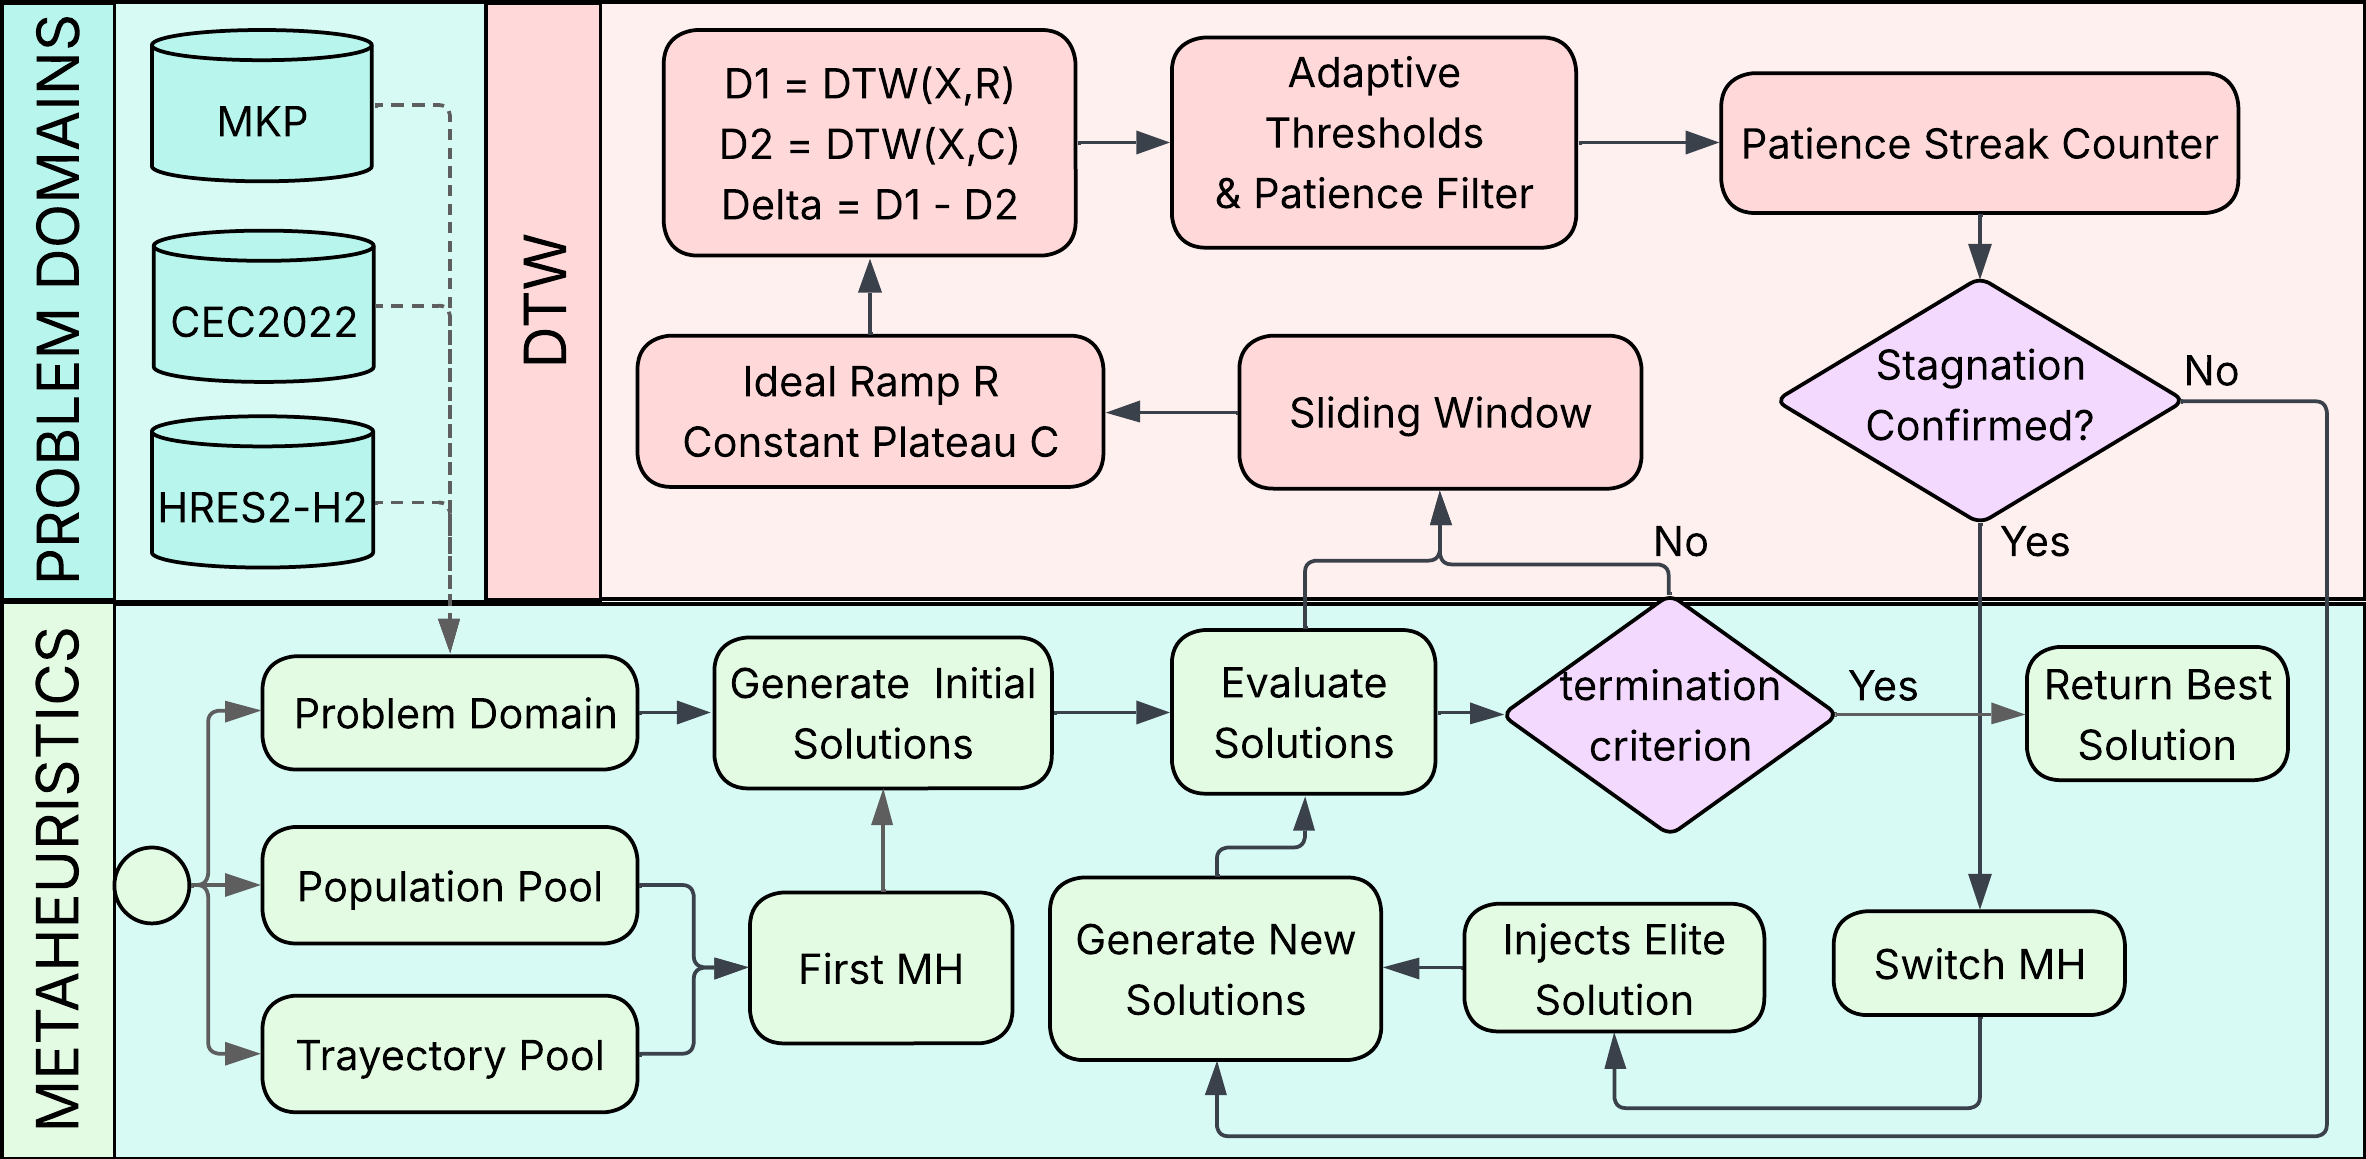
\includegraphics[width=\textwidth,height=6.15cm,keepaspectratio]{fig/Diagrama_flujo.png}
\end{frame}

% -----------------------------------------------------------------------------
\begin{frame}{DTW y DDTW: misma lógica, distinta señal}
  \begin{columns}[T,onlytextwidth]
    \column{0.46\textwidth}
      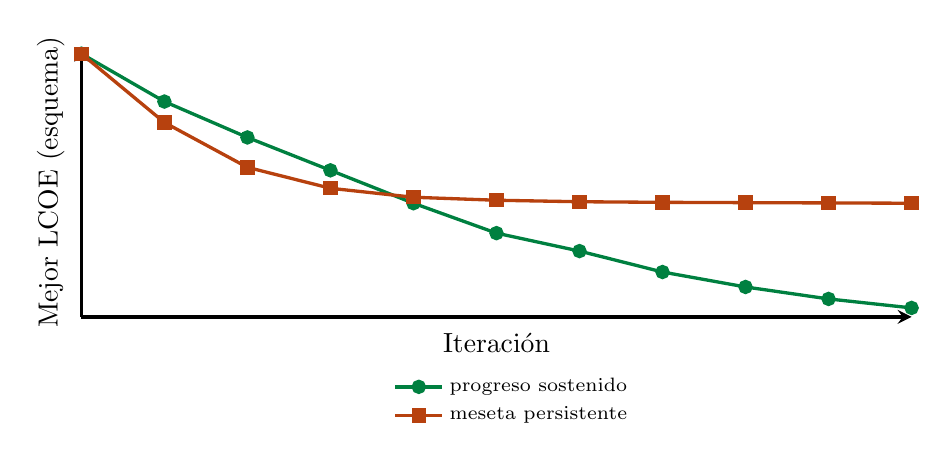
\begin{tikzpicture}
        \begin{axis}[
          width=\linewidth,height=5.0cm,
          axis lines=left,
          xlabel={Iteración},ylabel={Mejor LCOE (esquema)},
          xmin=0,xmax=10,ymin=0.12,ymax=1.02,
          xtick=\empty,ytick=\empty,
          legend style={draw=none,fill=none,font=\scriptsize,at={(0.52,-0.18)},anchor=north},
          line width=1.2pt
        ]
          \addplot[color=GreenH,mark=*] coordinates {(0,1.0)(1,.84)(2,.72)(3,.61)(4,.50)(5,.40)(6,.34)(7,.27)(8,.22)(9,.18)(10,.15)};
          \addlegendentry{progreso sostenido}
          \addplot[color=PUCVRed,mark=square*] coordinates {(0,1.0)(1,.77)(2,.62)(3,.55)(4,.52)(5,.51)(6,.505)(7,.503)(8,.502)(9,.501)(10,.50)};
          \addlegendentry{meseta persistente}
        \end{axis}
      \end{tikzpicture}

    \column{0.50\textwidth}
      \begin{block}{Dos referencias para la misma ventana $X$}
        \footnotesize
        $r$: rampa de progreso. \qquad $c$: señal constante o meseta.
        \[
          D_{\mathrm{prog}}=d(X,r),\qquad
          D_{\mathrm{mes}}=d(X,c)
        \]
      \end{block}

      \footnotesize
      \begin{tabularx}{\linewidth}{>{\bfseries\color{PUCVBlueDark}}p{1.1cm} X}
        \toprule
        Variante & Señal que compara \\
        \midrule
        DTW & niveles de $X$, $r$ y $c$ \\
        DDTW & primeras diferencias $\nabla X$, $\nabla r$ y $\nabla c$ \\
        \bottomrule
      \end{tabularx}

      \vspace{0.18cm}
      

  \end{columns}
\end{frame}

% -----------------------------------------------------------------------------
\begin{frame}{Banda Sakoe--Chiba: limitar el alineamiento}
  \begin{columns}[T,onlytextwidth]
    \column{0.52\textwidth}
      \centering
      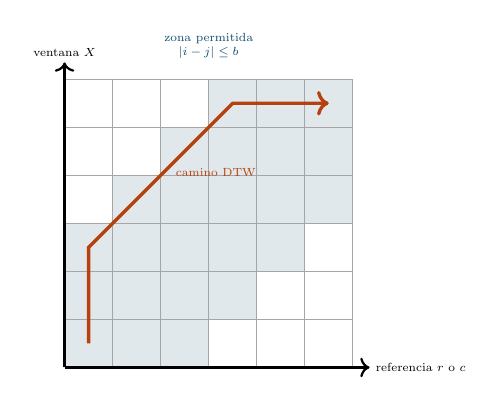
\begin{tikzpicture}[scale=0.61,transform shape]
        % Región permitida: |i-j| <= 2 para el ejemplo de seis puntos.
        \foreach \i in {0,...,5}{
          \foreach \j in {0,...,5}{
            \pgfmathtruncatemacro{\dif}{abs(\i-\j)}
            \ifnum\dif<3
              \fill[PUCVBlue!13] (\j,\i) rectangle ++(1,1);
            \fi
          }
        }
        \draw[step=1,gray!70] (0,0) grid (6,6);
        \draw[->,thick] (0,0) -- (6.35,0) node[right,font=\scriptsize]{referencia $r$ o $c$};
        \draw[->,thick] (0,0) -- (0,6.35) node[above,font=\scriptsize]{ventana $X$};
        \draw[PUCVRed,very thick,->]
          (0.5,0.5) -- (0.5,1.5) -- (0.5,2.5)
          -- (1.5,3.5) -- (2.5,4.5) -- (3.5,5.5)
          -- (4.5,5.5) -- (5.5,5.5);
        \node[font=\scriptsize,PUCVBlueDark,align=center] at (3.0,6.70) {zona permitida\\$|i-j|\leq b$};
        \node[font=\scriptsize,PUCVRed] at (3.15,4.05) {camino DTW};
      \end{tikzpicture}

      {\tiny Azul: celdas que el algoritmo puede visitar. Rojo: camino óptimo del ejemplo.}

    \column{0.44\textwidth}
      \begin{block}{Banda permitida}
        \scriptsize
        Solo visita celdas con $|i-j|\leq b$; así evita alineamientos entre puntos muy lejanos.
      \end{block}

      \begin{exampleblock}{Recurrencia DTW implementada}
        \tiny
        $C_{ij}=|X_i-Y_j|$, con
        $D_{0,0}=0$ y $D_{i,0}=D_{0,j}=\infty$.
        \[
          \boxed{D_{ij}=C_{ij}+\min\!\left\{
          D_{i-1,j},\;D_{i,j-1},\;D_{i-1,j-1}\right\}}
        \]
        Tres movimientos: avanza $X$, avanza $Y$ o avanzan ambas series.
      \end{exampleblock}

      \begin{alertblock}{Ejemplo e implementación}
        \tiny
        $W=6$, $b=2$: $(3,5)$ permitido; $(1,5)$ prohibido.\\[-1pt]
      \end{alertblock}
  \end{columns}
\end{frame}

% -----------------------------------------------------------------------------
\begin{frame}{Ejemplo numérico: DTW con los tres movimientos}
  \tiny
  \begin{block}{Misma forma, distinto ritmo}
    \centering
    $X=[.50,.50,.50,.56,.60,.65]$ \;(\text{ventana observada})\qquad
    $r=[.50,.55,.60,.64,.65,.65]$ \;(\text{progreso})\qquad b=2
  \end{block}

  \begin{columns}[T,onlytextwidth]
    \column{0.56\textwidth}
      \begin{exampleblock}{Costos locales $C_{ij}=|X_i-r_j|$}
        \centering
        {\setlength{\tabcolsep}{1.8pt}\renewcommand{\arraystretch}{1.10}
        \begin{tabular}{c|cccccc}
          & $r_1=.50$ & $r_2=.55$ & $r_3=.60$ & $r_4=.64$ & $r_5=.65$ & $r_6=.65$\\ \hline
          $X_1=.50$ & \cellcolor{best!22}0 & .05 & .10 & \cellcolor{gray!10}-- & \cellcolor{gray!10}-- & \cellcolor{gray!10}--\\
          $X_2=.50$ & \cellcolor{best!22}0 & .05 & .10 & .14 & \cellcolor{gray!10}-- & \cellcolor{gray!10}--\\
          $X_3=.50$ & \cellcolor{best!22}0 & .05 & .10 & .14 & .15 & \cellcolor{gray!10}--\\
          $X_4=.56$ & \cellcolor{gray!10}-- & \cellcolor{best!22}.01 & .04 & .08 & .09 & .09\\
          $X_5=.60$ & \cellcolor{gray!10}-- & \cellcolor{gray!10}-- & \cellcolor{best!22}0 & .04 & .05 & .05\\
          $X_6=.65$ & \cellcolor{gray!10}-- & \cellcolor{gray!10}-- & \cellcolor{gray!10}-- & \cellcolor{best!22}.01 & \cellcolor{best!22}0 & \cellcolor{best!22}0
        \end{tabular}}

        {\scriptsize Verde: camino óptimo. Gris: celdas fuera de la banda $b=2$.}
      \end{exampleblock}

    \column{0.41\textwidth}
      \begin{exampleblock}{Camino óptimo}
        \tiny
        \textbf{Vertical:}
        $(1,1)\downarrow(2,1)\downarrow(3,1)$;\quad costo $=0$.\\[3pt]
        \textbf{Diagonal:}
        $(3,1)\searrow(4,2)\searrow(5,3)\searrow(6,4)$;\\[-1pt]
        \hfill costo $=0.01+0+0.01=0.02$.\\[3pt]
        \textbf{Horizontal:}
        $(6,4)\rightarrow(6,5)\rightarrow(6,6)$;\quad costo $=0$.\\[5pt]
        \centering
        $\boxed{D_{\mathrm{prog}}=\operatorname{DTW}(X,r)=0.02}$
      \end{exampleblock}
  \end{columns}

  \begin{alertblock}{Comparación con la meseta}
    \centering
    $c=[.50,.50,.50,.50,.50,.50]$,\quad
    $D_{\mathrm{mes}}=\operatorname{DTW}(X,c)=0.31$,\quad
    $\delta=0.02-0.31=-0.29$
    $\Rightarrow$ \good{más cerca del progreso}.
  \end{alertblock}
\end{frame}

% -----------------------------------------------------------------------------
\begin{frame}{El discriminante $\delta$: progreso frente a meseta}
  \begin{columns}[T,onlytextwidth]
    \column{0.48\textwidth}
      \begin{block}{Diferencia implementada}
        \small
        \centering
        $D_{\mathrm{prog}}=D_1$ \quad y \quad $D_{\mathrm{mes}}=D_2$
        \vspace{0.08cm}

        $\boxed{\delta=D_{\mathrm{prog}}-D_{\mathrm{mes}}=D_1-D_2}$
      \end{block}

      \begin{block}{Cómo interpretar el signo}
        \footnotesize
        \begin{itemize}
          \item $\delta<0$: más cerca del \good{progreso}.
          \item $\delta\approx0$: evidencia ambigua; observar.
          \item $\delta>0$: más cerca de la \risk{meseta}.
        \end{itemize}
      \end{block}

      {\scriptsize\textbf{Ejemplo:} $0.80-0.20=0.60$; la ventana se parece más a la meseta.}

    \column{0.48\textwidth}
      \begin{alertblock}{Condiciones de estancamiento}
        \tiny
        El cambio se considera solo si se cumplen las tres condiciones:
        \begin{enumerate}
          \item \textbf{Sin mejora:} $\mathrm{sin\_mejora}\geq15$.
          \item \textbf{Cercanía a meseta:} $D_{\mathrm{mes}}\leq\theta_c$.
          \item \textbf{Alejamiento del progreso:} $D_{\mathrm{prog}}\geq\theta_r$
          o $\delta\geq\theta_\delta$.
        \end{enumerate}
        Además, deben confirmarse durante $3$ actualizaciones consecutivas.
      \end{alertblock}

      \begin{block}{Dónde cambia DDTW}
        \scriptsize
        DDTW usa las mismas dos distancias y el mismo $\delta$, pero sobre
        $\nabla x_t=x_t-x_{t-1}$. DTW compara niveles; DDTW compara cambios.
      \end{block}

      {\tiny Benchmark HRES2--H$_2$: $W=40$; banda $\approx4$; \texttt{use\_ddtw=True}; $patience=3$.\\
      Umbrales adaptativos P30/P70.}

  \end{columns}
\end{frame}

% -----------------------------------------------------------------------------
\begin{frame}{Conjunto de metaheurísticas}
  \begin{columns}[T,onlytextwidth]
    \column{0.49\textwidth}
      {\large\key{Poblacionales}}

      \vspace{0.16cm}
      \begin{tabularx}{\linewidth}{>{\bfseries}p{0.95cm} X}
        GA  & evolución y recombinación \\
        PSO & movimiento social de partículas \\
        GWO & jerarquía de búsqueda \\
        WOA & rodeo y trayectoria espiral \\
        EHO & dinámica de manada \\
        ACO & muestreo desde memoria colectiva \\
      \end{tabularx}

      \vspace{0.25cm}
      \good{Función dominante:} diversificación y exploración global.

    \column{0.47\textwidth}
      {\large\key{De trayectoria}}

      \vspace{0.16cm}
      \begin{tabularx}{\linewidth}{>{\bfseries}p{0.95cm} X}
        SA  & aceptación probabilística \\
        TS  & memoria tabú y aspiración \\
        ILS & perturbación y búsqueda local \\
        VNS & cambio sistemático de vecindad \\
      \end{tabularx}

      \vspace{1.1cm}
      \good{Función dominante:} intensificación y refinamiento local.

    
  \end{columns}
\end{frame}

% -----------------------------------------------------------------------------
\begin{frame}{Comunicación entre solucionadores}
  \begin{columns}[T,onlytextwidth]
    \column{0.56\textwidth}
      \begin{enumerate}
        \item Una metaheurística ejecuta un bloque de iteraciones.
        \item DTW/DDTW revisa si el mejor LCOE sigue mejorando.
        \item Si detecta estancamiento, termina ese bloque.
        \item Se guarda la mejor solución encontrada hasta ese momento.
        \item Se elige otra metaheurística y se le entrega esa solución para comenzar.
      \end{enumerate}

    \column{0.40\textwidth}
      \begin{exampleblock}{¿Cómo se hace el cambio?}
        \centering
        \small
        \textbf{MH activa}\\
        $\downarrow$\\[-0.05cm]
        alerta de estancamiento\\[-0.05cm]
        $\downarrow$\\[-0.05cm]
        \textbf{otra MH}
        
        \vspace{0.12cm}
        {\scriptsize Ejemplo: PSO $\rightarrow$ SA $\rightarrow$ ABC.}\\[0.08cm]
        La mejor solución se conserva y se entrega al receptor.
      \end{exampleblock}

      \begin{block}{Warm start, en simple}
        \scriptsize
        Recibe la mejor solución; no parte de cero.\\
        Población: inyección más candidatos nuevos.\\
        Alternancia poblacional $\rightarrow$ trayectoria $\rightarrow$ poblacional;
        DTW/DDTW decide.
      \end{block}

  \end{columns}
\end{frame}

\section{3. Modelo HRES2--H$_2$ implementado}

\begin{frame}[plain]
  \centering
  \vfill
  {\usebeamerfont{title}\color{primary}3. Modelo HRES2--H$_2$ implementado}\\[0.6em]
  {\color{accent}\rule{4.2cm}{2.2pt}}
  \vfill
\end{frame}

% -----------------------------------------------------------------------------
\begin{frame}{WPEB publicado vs. implementación HRES2--H$_2$}
  \tiny
  \setlength{\tabcolsep}{3.5pt}
  \renewcommand{\arraystretch}{1.18}
  \begin{tabularx}{\textwidth}{>{\bfseries\color{PUCVBlueDark}}p{2.85cm} X X}
    \toprule
    Parámetro & WPEB de Li et al. (2024) & Implementación HRES2--H$_2$ \\
    \midrule
    Variables de diseño
      & Razones eólica/electrólisis; capacidades continuas.
      & $\mathbf{x}=[P_{\mathrm{WT}},N_{\mathrm{el}},P_{\mathrm{bat}},\tau_{\mathrm{bat}}]^T$; mixto. \\
    Renovables
      & $P_{\mathrm{WT}}+P_{\mathrm{PV}}=200$ MW.
      & Misma capacidad total fija; $P_{\mathrm{PV}}=200-P_{\mathrm{WT}}$ MW. \\
    Electrolizador
      & Estación continua; caso óptimo E95 (95 MW).
      & $N_{\mathrm{el}}\in\{10,\ldots,20\}$ módulos de 5 MW. \\
    BESS
      & Fijo: $P_{\mathrm{bat}}=0.30P_{\mathrm{el}}$ y 1 h.
      & $P_{\mathrm{bat}}\in\{0,5,\ldots,50\}$ MW; $\tau_{\mathrm{bat}}\in\{1,2,4\}$ h. \\
    Simulación y restricción
      & Despacho horario de 8.760 h; $\mathrm{AGSR}\leq20\%$.
      & Mismo horizonte y AGSR; penalización de diseños inviables. \\
    Optimización
      & Grid search + descenso de gradiente; minimiza LCOE.
      & DTW/DDTW: cambia solucionador, transfiere incumbente y reporta LCOH. \\
    \bottomrule
  \end{tabularx}

  \vspace{0.1cm}
  \begin{exampleblock}{Diferencia que se quiere medir}
    La física se conserva; la extensión añade variables discretas y cooperación adaptativa entre metaheurísticas.
  \end{exampleblock}

  \vspace{0.04cm}
  {\tiny\color{Muted}Referencia: W190--P10--E95--B30, LCOE $=0.2692$ CNY/kWh.}
\end{frame}

% -----------------------------------------------------------------------------
\begin{frame}{HRES--H$_2$: qué se dimensiona}
  \centering
  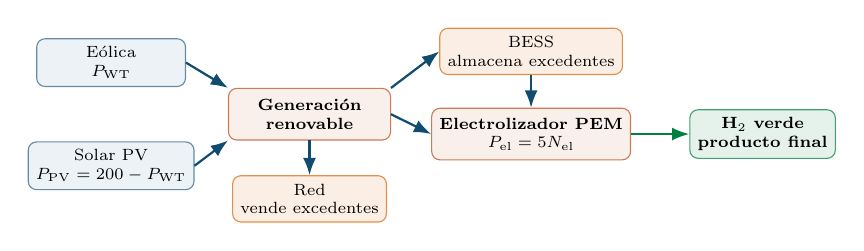
\begin{tikzpicture}[
    scale=0.84,transform shape,
    source/.style={draw=PUCVBlue!65,fill=PUCVLight,rounded corners=3pt,
      minimum width=2.25cm,minimum height=0.70cm,align=center,font=\scriptsize},
    core/.style={draw=PUCVRed!70,fill=PUCVRed!8,rounded corners=3pt,
      minimum width=2.45cm,minimum height=0.78cm,align=center,font=\scriptsize\bfseries},
    store/.style={draw=WarmGold!85,fill=WarmGold!12,rounded corners=3pt,
      minimum width=2.25cm,minimum height=0.70cm,align=center,font=\scriptsize},
    product/.style={draw=GreenH!75,fill=GreenH!10,rounded corners=3pt,
      minimum width=2.20cm,minimum height=0.70cm,align=center,font=\scriptsize\bfseries},
    flow/.style={-{Latex[length=2.2mm]},thick,color=PUCVBlue},
    hflow/.style={-{Latex[length=2.2mm]},thick,color=GreenH}
  ]
    \node[source] (wind) at (0,0.78) {Eólica\\$P_{\mathrm{WT}}$};
    \node[source] (pv) at (0,-0.78) {Solar PV\\$P_{\mathrm{PV}}=200-P_{\mathrm{WT}}$};
    \node[core] (renew) at (3.0,0) {Generación\\renovable};
    \node[store] (bat) at (6.35,0.95) {BESS\\almacena excedentes};
    \node[core] (ely) at (6.35,-0.30) {Electrolizador PEM\\$P_{\mathrm{el}}=5N_{\mathrm{el}}$};
    \node[store] (grid) at (3.0,-1.28) {Red\\vende excedentes};
    \node[product] (h2) at (9.85,-0.30) {H$_2$ verde\\producto final};

    % Entradas renovables y rutas de despacho, sin etiquetas sobrepuestas.
    \draw[flow] (wind.east) -- (renew.north west);
    \draw[flow] (pv.east) -- (renew.south west);
    \draw[flow] (renew.east) -- (ely.west);
    \draw[flow] (renew.north east) -- (bat.west);
    \draw[flow] (renew.south) -- (grid.north);
    \draw[flow] (bat.south) -- (ely.north);
    \draw[hflow] (ely.east) -- (h2.west);
  \end{tikzpicture}

  \vspace{-0.02cm}
  {\scriptsize\textcolor{PUCVBlue}{\bfseries Flujo de energía:} renovables, batería y red
  \hspace{0.7cm} \textcolor{GreenH}{\bfseries Flujo de producto:} electrolizador $\rightarrow$ H$_2$}

  \vspace{0.12cm}
  \begin{minipage}{0.65\textwidth}
    \begin{block}{Variables que realmente optimiza el algoritmo}
      \tiny
      \renewcommand{\arraystretch}{1.03}
      \begin{tabularx}{\linewidth}{>{\bfseries\color{PUCVBlueDark}}p{1.35cm} X >{\raggedleft\arraybackslash}p{2.2cm}}
        \toprule
        Variable & Qué representa & Dominio \\
        \midrule
        $P_{\mathrm{WT}}$ & potencia eólica instalada & $0$--$200$ MW \\
        $N_{\mathrm{el}}$ & módulos PEM de 5 MW & $10$--$20$ módulos \\
        $P_{\mathrm{bat}}$ & potencia máxima BESS & $0$--$50$ MW, pasos de 5 \\
        $\tau_{\mathrm{bat}}$ & duración nominal BESS & $1$, $2$ o $4$ h \\
        \bottomrule
      \end{tabularx}
    \end{block}
  \end{minipage}
\end{frame}

% -----------------------------------------------------------------------------
\begin{frame}{Generación renovable horaria}
  \begin{columns}[T,onlytextwidth]
    \column{0.49\textwidth}
      \begin{block}{Generación eólica}
        \scriptsize
        La velocidad del viento determina el factor horario $f_{\mathrm{WT}}(t)$:
        \[
          f_{\mathrm{WT}}(t)=
          \begin{cases}
            0, & v<v_i\ \text{o}\ v\geq v_o,\\
            \dfrac{v^3-v_i^3}{v_r^3-v_i^3},
            & v_i\leq v<v_r,\\
            1, & v_r\leq v<v_o.
          \end{cases}
        \]
        $v_i=2.5$, $v_r=10.5$ y $v_o=25$ m/s. La potencia generada es
        $P_{\mathrm{WT}}f_{\mathrm{WT}}(t)$; la turbina nominal es de 5 MW.
      \end{block}

    \column{0.49\textwidth}
      \begin{exampleblock}{Generación fotovoltaica}
        \scriptsize
        La irradiancia es el factor principal de la generación solar.\vspace{-0.04cm}
        \[
          P_{\mathrm{PV}}^{\mathrm{gen}}(t)=
          P_{\mathrm{PV}}\,g(t)\,\underbrace{0.90}_{\text{pérdidas}}
          \underbrace{C_T(t)}_{\text{temperatura}}
        \]
        \begin{itemize}
          \item $g(t)$ representa la irradiancia horaria: de noche es cero.
          \item $C_T(t)$ reduce el rendimiento cuando la celda se calienta.
          \item El factor se limita al intervalo $[0,1]$.
        \end{itemize}
        \vspace{-0.08cm}
        \scriptsize $NOCT=47^\circ$C, $\gamma_T=-0.5\%/^\circ$C$;$
        $0.90$ representa pérdidas del sistema.
      \end{exampleblock}
  \end{columns}

  \vspace{0.06cm}
  \centering
  \destacado{Potencia disponible cada hora:}
  \[
    P_{\mathrm{gen}}(t)=P_{\mathrm{WT}}f_{\mathrm{WT}}(t)+P_{\mathrm{PV}}f_{\mathrm{PV}}(t)
    \leq P_{\mathrm{WT}}+P_{\mathrm{PV}}=200\,\mathrm{MW}.
  \]
  {\scriptsize $P_{\mathrm{WT}}$ y $P_{\mathrm{PV}}$ son capacidades instaladas, fijas las 8760 h;
  $f_{\mathrm{WT}}(t),f_{\mathrm{PV}}(t)\in[0,1]$ varían con el clima.}
\end{frame}

% -----------------------------------------------------------------------------
\begin{frame}{HRES--H$_2$: cómo opera cada hora}
  \begin{columns}[T,onlytextwidth]
    \column{0.56\textwidth}
      \begin{enumerate}
        \item Calcular $P_{\mathrm{gen}}(t)=P_{\mathrm{WT}}(t)+P_{\mathrm{PV}}(t)$ a partir del clima.
        \item Si $P_{\mathrm{gen}}(t)\geq0.30P_{\mathrm{el}}$, alimentar el PEM hasta $P_{\mathrm{el}}$.
        \item Si no se alcanza ese mínimo, descargar BESS si hay energía; si no, detener el electrolizador esa hora.
        \item El excedente carga el BESS hasta $SOC\leq P_{\mathrm{bat}}\tau_{\mathrm{bat}}$; lo restante se vende a la red.
      \end{enumerate}

    \column{0.39\textwidth}
      \begin{block}{Energía anual que recibe el PEM}
        \scriptsize
        \[
          E_{\mathrm{el,annual}}=
          \sum_{t=1}^{8760}P_{\mathrm{el,usada}}(t)\,\Delta t
        \]
        \scriptsize $P_{\mathrm{el,usada}}(t)$ es la potencia que realmente consume el PEM en la hora $t$; con $\Delta t=1$ h, la suma queda en MWh/año.
      \end{block}
      \vspace{0.15cm}
      \small La simulación recorre las 8.760 horas. La carga y descarga usan $\eta_{\mathrm{ch}}=\eta_{\mathrm{dis}}=\sqrt{0.90}\approx0.9487$.
  \end{columns}
\end{frame}

% -----------------------------------------------------------------------------
\begin{frame}{De electricidad renovable a producción de H$_2$}
  \begin{columns}[T,onlytextwidth]
    \column{0.48\textwidth}
      \begin{block}{1. Energía que realmente usó el PEM}
        \small
        \[
          E_{\mathrm{el,annual}}=
          \sum_{t=1}^{8760}P_{\mathrm{el,usada}}(t)\,\Delta t
        \]
        \footnotesize
        $P_{\mathrm{el,usada}}(t)$ es la potencia realmente consumida en la hora $t$ [MW]. Como $\Delta t=1$ h, la suma da $E_{\mathrm{el,annual}}$ en MWh/año: se usa el consumo del despacho, no $P_{\mathrm{el}}\times8760$.
      \end{block}

    \column{0.48\textwidth}
      \begin{exampleblock}{2. Conversión de energía a masa}
        \small
        \[
          m_{\mathrm{H_2}}=
          \frac{E_{\mathrm{el,annual}}\cdot1000\cdot\eta_{\mathrm{el}}}
          {HHV_{\mathrm{H_2}}}
        \]
        \footnotesize
        $m_{\mathrm{H_2}}$: kg producidos por año.\\
        $\eta_{\mathrm{el}}=0.75$: eficiencia, sin unidades.\\
        $HHV_{\mathrm{H_2}}=39.4$ kWh/kg: energía por kg de H$_2$.\\
        $1000$: convierte MWh a kWh.
      \end{exampleblock}
  \end{columns}

  
\end{frame}

% -----------------------------------------------------------------------------
\begin{frame}{HRES--H$_2$: objetivos y restricciones}
  \begin{columns}[T,onlytextwidth]
    \column{0.48\textwidth}
      \key{Costo nivelado de electricidad (LCOE)}
      \[
        \mathrm{LCOE}=\frac{\mathrm{NPC}\cdot\mathrm{CRF}}
        {E_{\mathrm{entregada,annual}}}
      \]
      {\scriptsize
      \begin{itemize}
        \setlength{\itemsep}{0.04cm}
        \item $NPC$: costo presente neto: CAPEX, reemplazos y operación/mantenimiento.
        \item $CRF$: factor que convierte el $NPC$ en costo anual equivalente:
        \(CRF=\frac{r(1+r)^N}{(1+r)^N-1}\).
        \item $r=4.35\%$: tasa de descuento real; $N=25$: años del proyecto.
        \item $E_{\mathrm{entregada,annual}}=1000(E_{\mathrm{el,annual}}+E_{\mathrm{grid,sales,annual}})$: energía anual contabilizada [kWh/año].
      \end{itemize}}

    \column{0.48\textwidth}
      \key{Restricciones y penalización}
      \begin{itemize}
        \item $P_{\mathrm{WT}}+P_{\mathrm{PV}}=200$ MW;
        \item dominios mixtos de $N_{\mathrm{el}}$, $P_{\mathrm{bat}}$ y $\tau_{\mathrm{bat}}$;
      \end{itemize}

      \begin{block}{Límite de exportación anual}
        \[
          \mathrm{AGSR}=
          \frac{\sum_{t=1}^{8760}P_{\mathrm{grid\_sales}}(t)}
          {\sum_{t=1}^{8760}P_{\mathrm{gen}}(t)}
          \leq0.20
        \]
      \end{block}

      {\footnotesize Si $\mathrm{AGSR}>0.20$, el modelo usa
      $f_{\mathrm{pen}}(\mathbf{x})=100+10\,\mathrm{AGSR}$.}

  \end{columns}
  \vfill
\end{frame}

% -----------------------------------------------------------------------------
\begin{frame}{Cómo se integra el optimizador con el HRES}
  \centering
  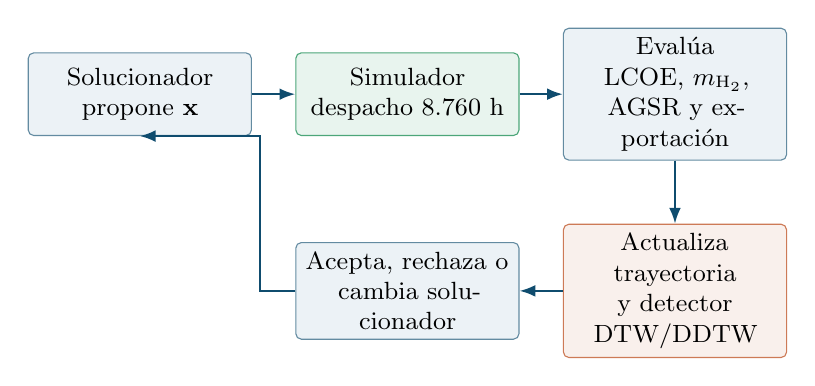
\begin{tikzpicture}[
    node distance=0.55cm and 0.55cm,
    integ/.style={draw=PUCVBlue!65,fill=PUCVLight,rounded corners=2pt,
      minimum height=1.05cm,text width=2.6cm,align=center,font=\small},
    sim/.style={draw=GreenH!70,fill=GreenH!9,rounded corners=2pt,
      minimum height=1.05cm,text width=2.6cm,align=center,font=\small},
    ctrl/.style={draw=PUCVRed!70,fill=PUCVRed!8,rounded corners=2pt,
      minimum height=1.05cm,text width=2.6cm,align=center,font=\small},
    flow/.style={-{Latex[length=2mm]},thick,color=PUCVBlue}
  ]
    \node[integ] (candidate) {Solucionador\\propone $\mathbf{x}$};
    \node[sim,right=of candidate] (dispatch) {Simulador\\despacho 8.760 h};
    \node[integ,right=of dispatch] (metrics) {Evalúa LCOE, $m_{\mathrm{H_2}}$,\\AGSR y exportación};
    \node[ctrl,below=0.8cm of metrics] (trace) {Actualiza trayectoria\\y detector DTW/DDTW};
    \node[integ,left=of trace] (next) {Acepta, rechaza o\\cambia solucionador};
    \draw[flow] (candidate) -- (dispatch);
    \draw[flow] (dispatch) -- (metrics);
    \draw[flow] (metrics) -- (trace);
    \draw[flow] (trace) -- (next);
    \draw[flow] (next.west) -| ++(-0.45,0) |- (candidate.south);
  \end{tikzpicture}

  \vspace{0.35cm}
  \begin{block}{Interfaz cooperativa}
    El HRES no recibe una metaheurística específica: recibe candidatos factibles, devuelve indicadores comparables y conserva el incumbente para la siguiente época.
  \end{block}
\end{frame}



% -----------------------------------------------------------------------------
\begin{frame}{Resultados HRES2--H$_2$: métricas y configuración}
  \scriptsize
  \begin{columns}[T,onlytextwidth]
    \column{0.54\textwidth}
      \begin{block}{31 corridas independientes}
        \setlength{\tabcolsep}{2.5pt}
        \renewcommand{\arraystretch}{1.35}
        \begin{tabularx}{\linewidth}{>{\bfseries}p{1.05cm} >{\centering\arraybackslash}p{1.45cm} >{\centering\arraybackslash}p{1.35cm} >{\centering\arraybackslash}p{1.2cm} X}
          \toprule
          Variante & LCOE medio & LCOH medio & $\sigma$ & Factibilidad / AGSR \\
          \midrule
          \rowcolor{PUCVLight}
          DTW & 0.267160 & 17.6314 & 0.000001 & 100\% / 20.00\% \\
          DDTW & 0.267160 & 17.6313 & 0.000005 & 100\% / 20.00\% \\
          \bottomrule
        \end{tabularx}
        \vspace{0.05cm}
        \centering Mejor LCOE observado: $0.267159$ CNY/kWh.
      \end{block}

    \column{0.42\textwidth}
      \begin{exampleblock}{Configuración común encontrada}
        \setlength{\tabcolsep}{3pt}
        \renewcommand{\arraystretch}{1.3}
        \begin{tabularx}{\linewidth}{>{\bfseries}p{2.3cm} >{\centering\arraybackslash}X}
          \toprule
          Eólica & 174.47 MW \\
          Solar PV & 25.53 MW \\
          Electrolizador & 70.0 MW (14 módulos) \\
          Batería & 50.0 MW / 4 h \\
          H$_2$ anual & 8,862,879.4 kg \\
          \bottomrule
        \end{tabularx}
      \end{exampleblock}
  \end{columns}

  
\end{frame}

% -----------------------------------------------------------------------------
\begin{frame}{HRES2--H$_2$: comparación con solucionadores base}
  \tiny
  \setlength{\tabcolsep}{3pt}
  \renewcommand{\arraystretch}{1.2}
  \begin{tabularx}{\textwidth}{>{\bfseries}p{2.05cm} >{\centering\arraybackslash}p{1.8cm} >{\centering\arraybackslash}p{1.8cm} >{\centering\arraybackslash}p{1.55cm} >{\centering\arraybackslash}p{1.35cm} X}
    \toprule
    Método & LCOE medio & Mejor LCOE & $\sigma$ & AGSR & Factibilidad \\
      & \scriptsize(CNY/kWh) & \scriptsize(CNY/kWh) & \scriptsize(CNY/kWh) & \scriptsize(\%) & \scriptsize(\%) \\
    \midrule
    \rowcolor{PUCVLight}Propuesto (DTW) & 0.267160 & 0.267159 & 0.000001 & 20.00 & 100.0 \\
    \rowcolor{PUCVLight}Propuesto (DDTW) & 0.267160 & 0.267159 & 0.000005 & 20.00 & 100.0 \\
    GWO & 0.268066 & 0.267160 & 0.002815 & 19.42 & 90.3 \\
    VNS & 0.267806 & 0.267159 & 0.002465 & 19.95 & 93.5 \\
    TS & 0.267188 & 0.267159 & 0.000038 & 19.99 & 96.8 \\
    ACO & 0.273288 & 0.267159 & 0.007584 & 18.95 & 93.5 \\
    ILS & 0.267184 & 0.267171 & 0.000023 & 19.98 & 96.8 \\
    PSO & 0.277289 & 0.274579 & 0.010939 & 19.85 & 83.8 \\
    WOA & 0.277227 & 0.276524 & 0.009567 & 19.70 & 87.1 \\
    EHO & 0.277728 & 0.276524 & 0.007382 & 19.92 & 80.6 \\
    SA & 0.286431 & 0.281339 & 0.013206 & 19.35 & 87.1 \\
    \bottomrule
  \end{tabularx}

  \vspace{0.25cm}
  \begin{block}{Lectura del resultado}
    En 31 corridas, DTW y DDTW combinan la menor media y el mejor LCOE, AGSR en el límite permitido y factibilidad completa; los métodos base muestran mayor variabilidad y/o diseños inviables.
  \end{block}
\end{frame}

% -----------------------------------------------------------------------------
\begin{frame}{Resultados HRES2--H$_2$: convergencia del pipeline DTW}
  \centering
  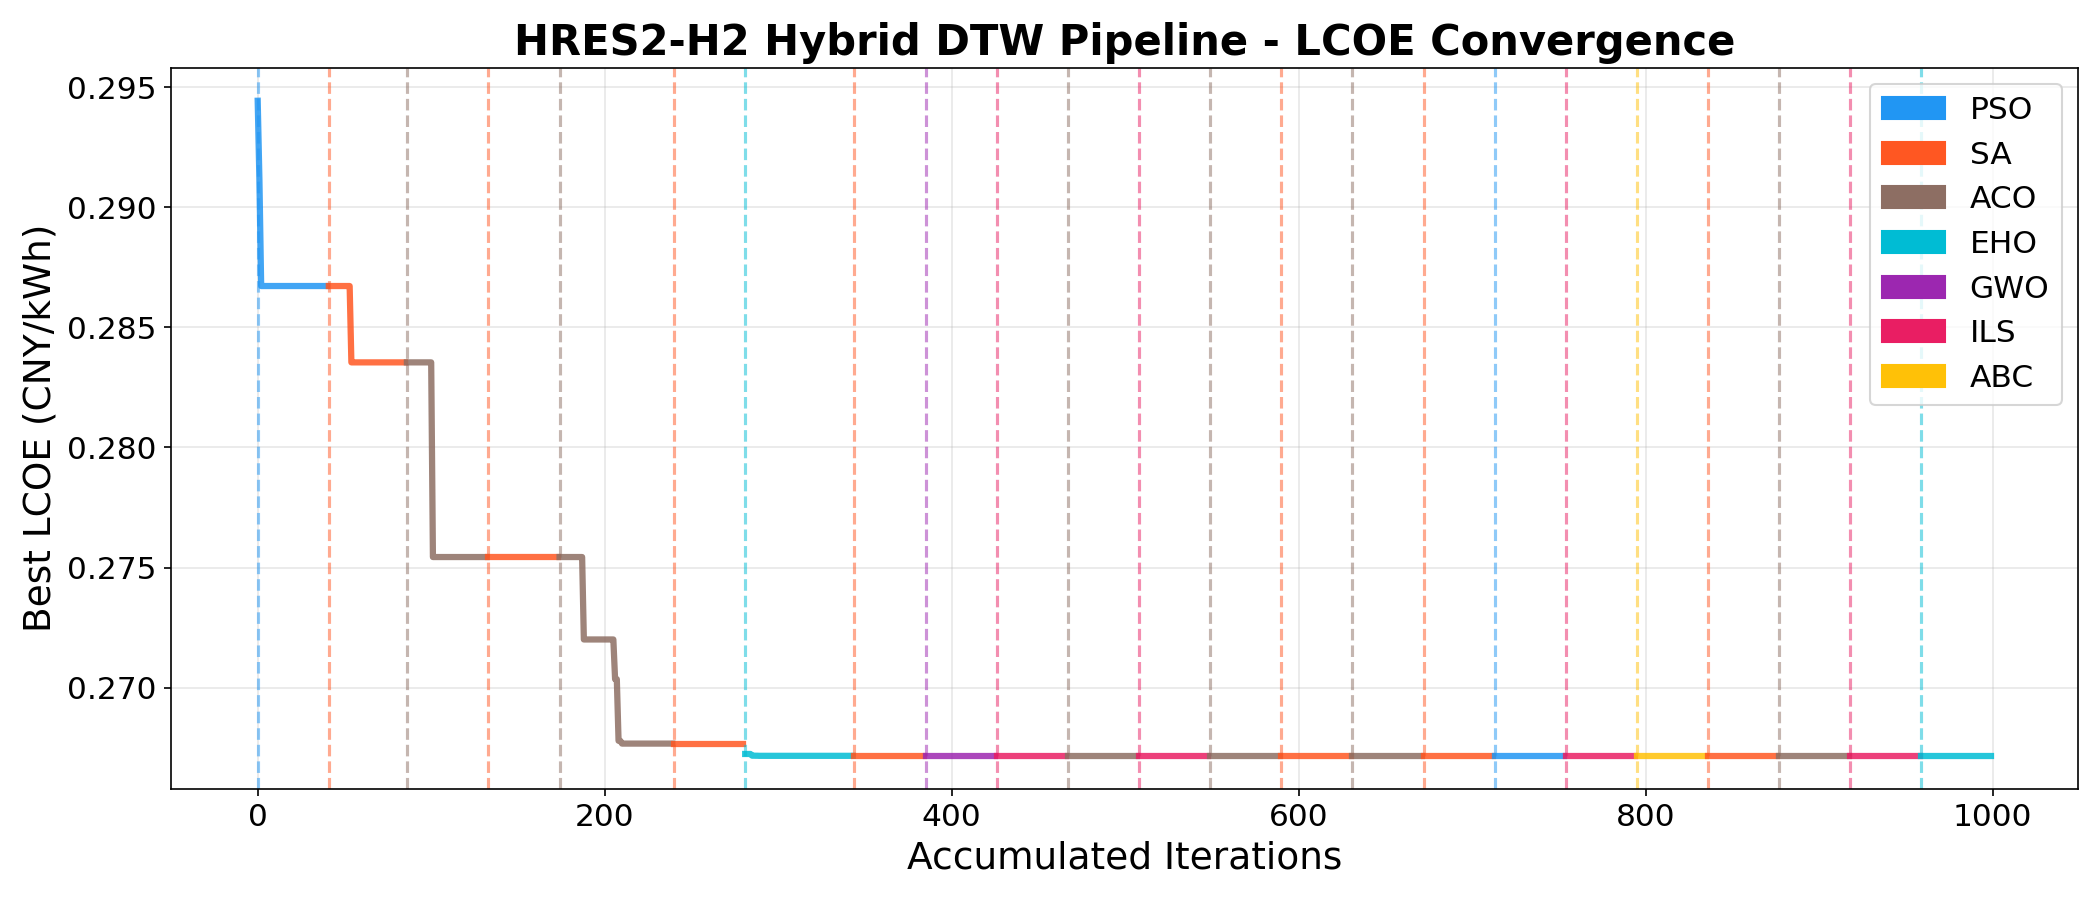
\includegraphics[width=0.98\textwidth,height=5.25cm,keepaspectratio]{fig/hres2_dtw_convergence.png}

  \vspace{0.08cm}
  {\scriptsize Las líneas verticales indican cambios de solucionador; el incumbente se conserva y la trayectoria se estabiliza en $0.267159$ CNY/kWh.}
\end{frame}

% -----------------------------------------------------------------------------
\begin{frame}{Resultados HRES2--H$_2$: convergencia del pipeline DDTW}
  \centering
  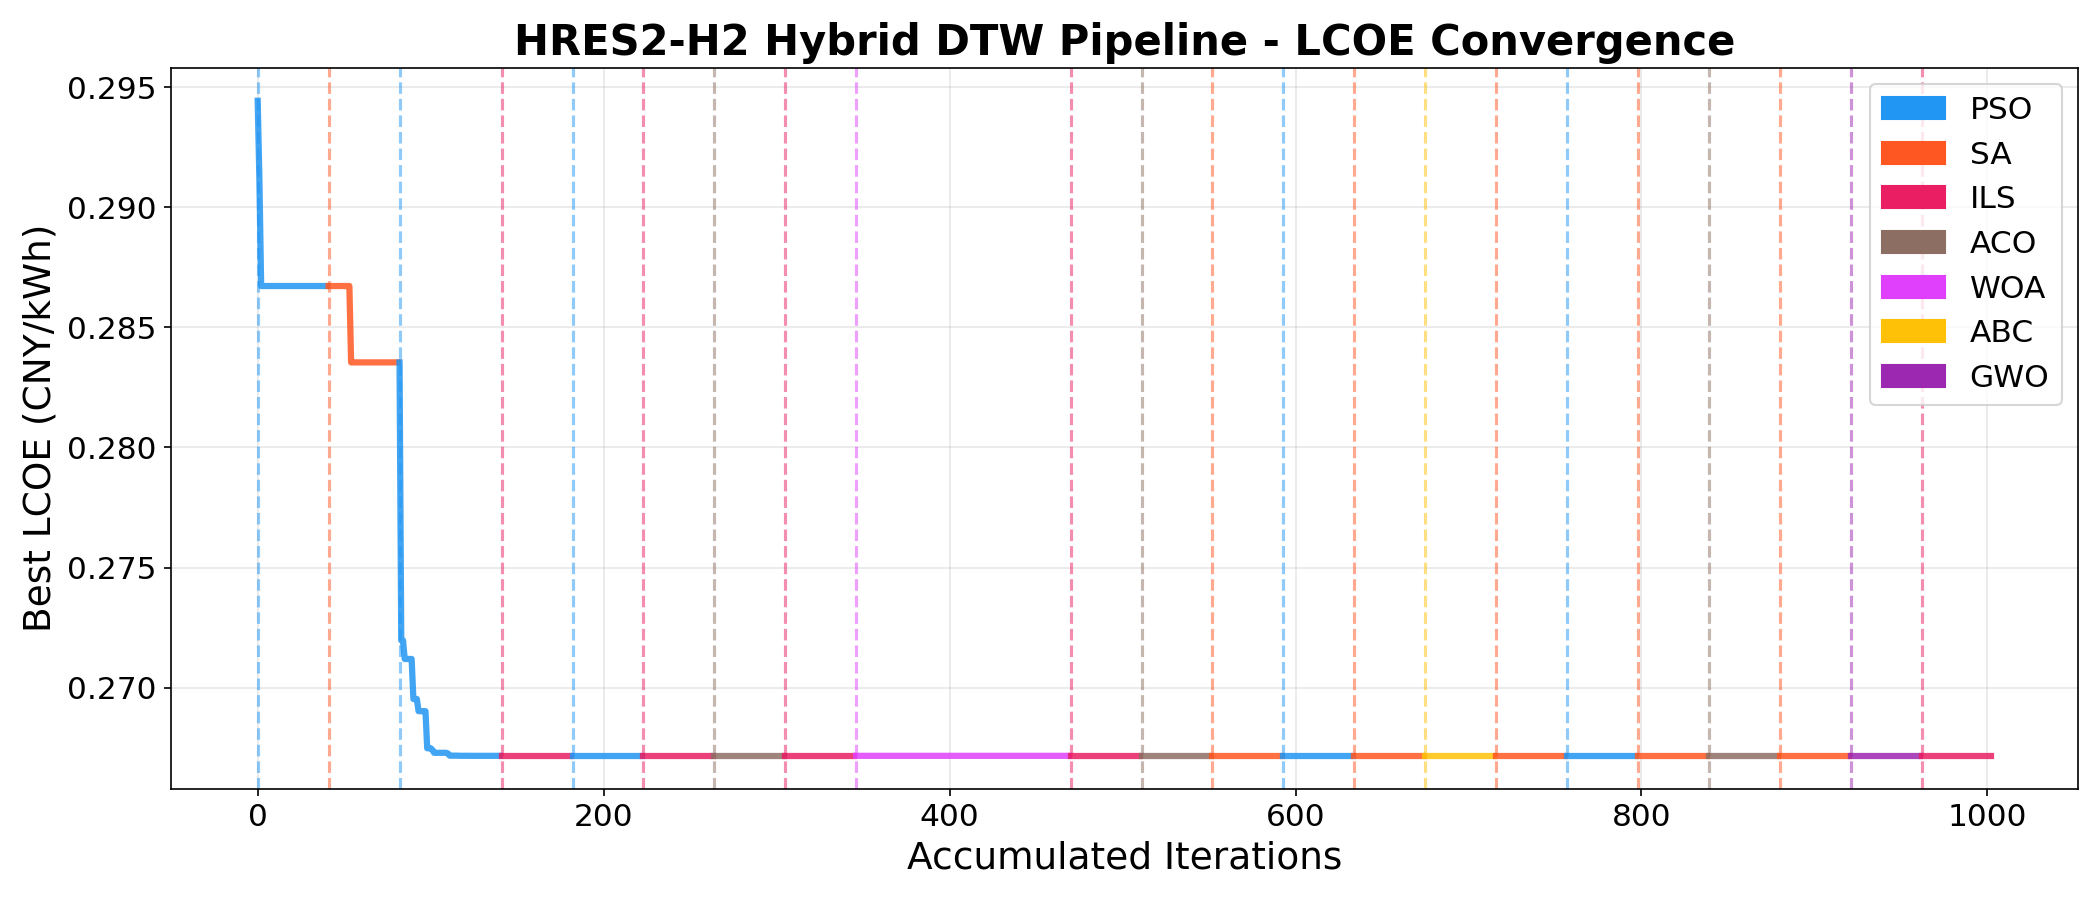
\includegraphics[width=0.98\textwidth,height=5.25cm,keepaspectratio]{fig/hres2_ddtw_convergence.png}

  \vspace{0.08cm}
  {\scriptsize La señal derivativa mantiene la misma solución final; los cambios de metaheurística aparecen sobre los mismos plateaus de la trayectoria.}
\end{frame}

\section{4. Validación y posicionamiento}

% -----------------------------------------------------------------------------
\begin{frame}{Posicionamiento frente al trabajo relacionado}
  \scriptsize
  \begin{tabularx}{\textwidth}{p{2.55cm} >{\centering\arraybackslash}p{1.25cm} >{\centering\arraybackslash}p{1.45cm} >{\centering\arraybackslash}p{1.4cm} X}
    \toprule
    Enfoque & Temporal & Cambia MH completa & Requiere aprendizaje & Señal principal \\
    \midrule
    Migración adaptativa & parcial & sí & no & mejora, diversidad o estancamiento \\
    Selección por trayectoria & sí & sí & sí & características y regresión de desempeño \\
    DAC con aprendizaje & sí & sí & sí & estado aprendido y recompensa \\
    \rowcolor{PUCVLight}
    \textbf{Propuesta DTW/DDTW} & \textbf{sí} & \textbf{sí} & \textbf{no} & \textbf{forma reciente del fitness incumbente} \\
    \bottomrule
  \end{tabularx}

  \vspace{0.42cm}
  \key{Diferenciación:} una señal interpretable, independiente del solucionador y sensible al orden temporal guía el intercambio entre metaheurísticas completas.

  \vfill
  \smallcite{mambrini2015design,jankovic2022trajectory,liu2025three,reijnen2025search}
\end{frame}

\section{5. Plan de trabajo}

% -----------------------------------------------------------------------------
\begin{frame}{Plan de trabajo (agosto--diciembre de 2026)}
  \centering
  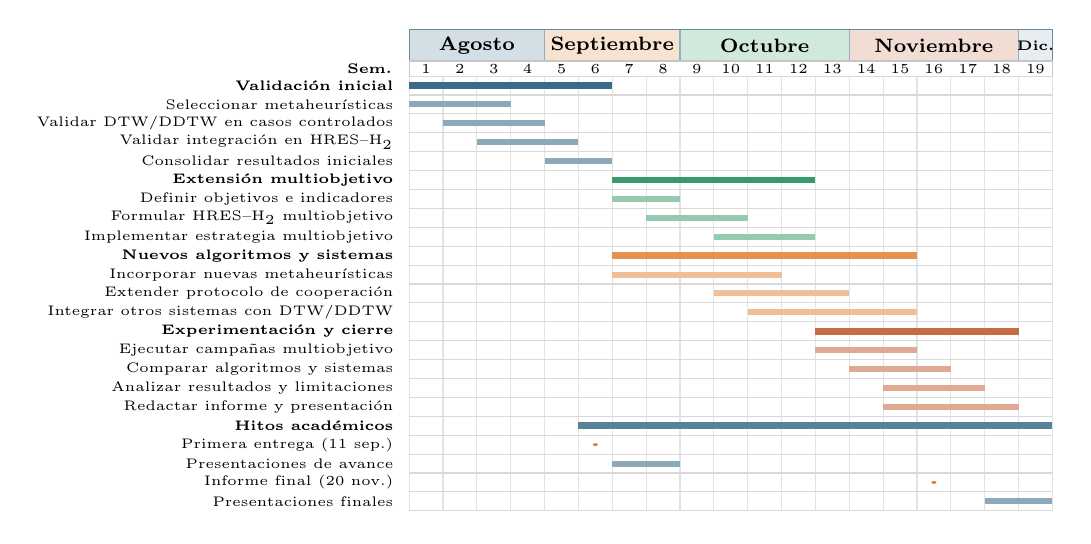
\begin{tikzpicture}[x=0.43cm,y=0.24cm]
    % Encabezado por meses y semanas, como en el formato anterior.
    \fill[primary!18] (0,0) rectangle (4,1.65);
    \fill[accent!22] (4,0) rectangle (8,1.65);
    \fill[best!18] (8,0) rectangle (13,1.65);
    \fill[warn!18] (13,0) rectangle (18,1.65);
    \fill[primary!10] (18,0) rectangle (19,1.65);
    \draw[primary!65] (0,0) rectangle (19,1.65);
    \draw[primary!45] (4,0)--(4,1.65) (8,0)--(8,1.65)
    (13,0)--(13,1.65) (18,0)--(18,1.65);
    \node[font=\scriptsize\bfseries] at (2,0.82) {Agosto};
    \node[font=\scriptsize\bfseries] at (6,0.82) {Septiembre};
    \node[font=\scriptsize\bfseries] at (10.5,0.82) {Octubre};
    \node[font=\scriptsize\bfseries] at (15.5,0.82) {Noviembre};
    \node[font=\tiny\bfseries] at (18.5,0.82) {Dic.};

    \draw[gray!45] (0,0) rectangle (19,-0.8);
    \node[font=\tiny\bfseries,anchor=east] at (-0.22,-0.4) {Sem.};
    \foreach \i in {1,...,19}{
      \pgfmathsetmacro{\xx}{\i-0.5}
      \node[font=\tiny] at (\xx,-0.4) {\i};
    }

    % Cuadrícula.
    \foreach \i in {0,...,19}{\draw[gray!22] (\i,-0.8)--(\i,-23.8);}
    \foreach \j in {0,...,23}{
      \pgfmathsetmacro{\yy}{-0.8-\j}
      \draw[gray!30] (0,\yy)--(19,\yy);
    }

    % Validación inicial: la selección de metaheurísticas es la primera tarea.
    \node[anchor=east,font=\tiny\bfseries] at (-0.18,-1.3) {Validación inicial};
    \fill[primary!82] (0,-1.48) rectangle (6,-1.12);
    \node[anchor=east,font=\tiny] at (-0.18,-2.3) {Seleccionar metaheurísticas};
    \fill[primary!48] (0,-2.46) rectangle (3,-2.14);
    \node[anchor=east,font=\tiny] at (-0.18,-3.3) {Validar DTW/DDTW en casos controlados};
    \fill[primary!48] (1,-3.46) rectangle (4,-3.14);
    \node[anchor=east,font=\tiny] at (-0.18,-4.3) {Validar integración en HRES--H$_2$};
    \fill[primary!48] (2,-4.46) rectangle (5,-4.14);
    \node[anchor=east,font=\tiny] at (-0.18,-5.3) {Consolidar resultados iniciales};
    \fill[primary!48] (4,-5.46) rectangle (6,-5.14);

    % Extensión multiobjetivo.
    \node[anchor=east,font=\tiny\bfseries] at (-0.18,-6.3) {Extensión multiobjetivo};
    \fill[best!78] (6,-6.48) rectangle (12,-6.12);
    \node[anchor=east,font=\tiny] at (-0.18,-7.3) {Definir objetivos e indicadores};
    \fill[best!42] (6,-7.46) rectangle (8,-7.14);
    \node[anchor=east,font=\tiny] at (-0.18,-8.3) {Formular HRES--H$_2$ multiobjetivo};
    \fill[best!42] (7,-8.46) rectangle (10,-8.14);
    \node[anchor=east,font=\tiny] at (-0.18,-9.3) {Implementar estrategia multiobjetivo};
    \fill[best!42] (9,-9.46) rectangle (12,-9.14);

    % Nuevas metaheurísticas y sistemas.
    \node[anchor=east,font=\tiny\bfseries] at (-0.18,-10.3) {Nuevos algoritmos y sistemas};
    \fill[accent!82] (6,-10.48) rectangle (15,-10.12);
    \node[anchor=east,font=\tiny] at (-0.18,-11.3) {Incorporar nuevas metaheurísticas};
    \fill[accent!48] (6,-11.46) rectangle (11,-11.14);
    \node[anchor=east,font=\tiny] at (-0.18,-12.3) {Extender protocolo de cooperación};
    \fill[accent!48] (9,-12.46) rectangle (13,-12.14);
    \node[anchor=east,font=\tiny] at (-0.18,-13.3) {Integrar otros sistemas con DTW/DDTW};
    \fill[accent!48] (10,-13.46) rectangle (15,-13.14);

    % Experimentación y cierre.
    \node[anchor=east,font=\tiny\bfseries] at (-0.18,-14.3) {Experimentación y cierre};
    \fill[warn!78] (12,-14.48) rectangle (18,-14.12);
    \node[anchor=east,font=\tiny] at (-0.18,-15.3) {Ejecutar campañas multiobjetivo};
    \fill[warn!45] (12,-15.46) rectangle (15,-15.14);
    \node[anchor=east,font=\tiny] at (-0.18,-16.3) {Comparar algoritmos y sistemas};
    \fill[warn!45] (13,-16.46) rectangle (16,-16.14);
    \node[anchor=east,font=\tiny] at (-0.18,-17.3) {Analizar resultados y limitaciones};
    \fill[warn!45] (14,-17.46) rectangle (17,-17.14);
    \node[anchor=east,font=\tiny] at (-0.18,-18.3) {Redactar informe y presentación};
    \fill[warn!45] (14,-18.46) rectangle (18,-18.14);

    % Hitos académicos; se elimina el hito de software.
    \node[anchor=east,font=\tiny\bfseries] at (-0.18,-19.3) {Hitos académicos};
    \fill[primary!70] (5,-19.48) rectangle (19,-19.12);
    \node[anchor=east,font=\tiny] at (-0.18,-20.3) {Primera entrega (11 sep.)};
    \fill[accent] (5.5,-20.3) circle (0.075);
    \node[anchor=east,font=\tiny] at (-0.18,-21.3) {Presentaciones de avance};
    \fill[primary!48] (6,-21.46) rectangle (8,-21.14);
    \node[anchor=east,font=\tiny] at (-0.18,-22.3) {Informe final (20 nov.)};
    \fill[accent] (15.5,-22.3) circle (0.075);
    \node[anchor=east,font=\tiny] at (-0.18,-23.3) {Presentaciones finales};
    \fill[primary!48] (17,-23.46) rectangle (19,-23.14);
  \end{tikzpicture}

  \vspace{0.02cm}
  {\tiny La primera entrega cierra la validación inicial (semana 6); luego se amplían el enfoque multiobjetivo, las metaheurísticas y los sistemas antes del informe final.}
\end{frame}

\section{6. Cierre}

% -----------------------------------------------------------------------------
\begin{frame}{Contribuciones esperadas}
  \begin{enumerate}
    \item Un detector de estancamiento que usa la forma temporal del fitness y funciona con metaheurísticas heterogéneas.
    \item Un protocolo de transferencia que preserva el incumbente y adapta la inicialización al algoritmo receptor.
    \item Un orquestador que alterna exploración y explotación según evidencia de la propia ejecución.
    \item Una validación gradual que conecta benchmarks discretos y continuos con el dimensionamiento HRES--H$_2$.
    \item Una extensión para estudiar compromisos económicos y ambientales mediante $\varepsilon$-restricción adaptativa.
  \end{enumerate}
\end{frame}

% -----------------------------------------------------------------------------
\appendix
\section{Referencias}
\begin{frame}[allowframebreaks]{Referencias citadas}
  \tiny
  \nocite{wolpert1997no,vega2021learning,akbulut2026artificial,talbi2021machine_tax,
    pei2025adaptive,adriaensen2022automated,jankovic2022trajectory,
    kostovska2022per,cenikj2026survey,berndt1994using,keogh2001derivative,
    mambrini2015design,liu2025three,reijnen2025search}
  \printbibliography[heading=none]
\end{frame}

\end{document}
